\chapter{Arhitektura i dizajn sustava}
\setlength{\headheight}{14.49998pt}		
		%\textbf{\textit{dio 1. revizije}}\\

		%\textit{ Potrebno je opisati stil arhitekture te identificirati: podsustave, preslikavanje na radnu platformu, spremišta podataka, mrežne protokole, globalni upravljački tok i sklopovsko-programske zahtjeve. Po točkama razraditi i popratiti odgovarajućim skicama:}
	%\begin{itemize}
		%\item 	\textit{izbor arhitekture temeljem principa oblikovanja pokazanih na predavanjima (objasniti zašto ste baš odabrali takvu arhitekturu)}
		%\item 	\textit{organizaciju sustava s najviše razine apstrakcije (npr. klijent-poslužitelj, baza podataka, datotečni sustav, grafičko sučelje)}
		%\item 	\textit{organizaciju aplikacije (npr. slojevi frontend i backend, MVC arhitektura) }
	%\end{itemize}

Stil arhitekture korišten za izradu ovog sustava je mješavina objektno usmjerenog arhitekturnog stila, te stila Model-Pogled-Nadglednik (MVC), kombinirajući prednosti obje arhitekture dok se istovremeno poništavaju njihovi nedostaci. Korisničko je sučelje izdvojeno od ostatka sustava, dok je općenit pristup rješenju objektno orijentiran. Sustav je podijeljen na tri glavna, manja podsustava:
\begin{itemize}
\item Bazu podataka
\item Obradu podataka (backend)
\item Korisničko sučelje (frontend)
\end{itemize}
Podsustav za obradu podataka jedini surađuje sa bazom, a podaci se ne spremaju nigdje osim u bazu. Korisničko sučelje pak sve podatke dobiva iz podsustava za obradu te se time osigurava integritet i dosljednost sustava.
Podsustav za obradu i korisničko sučelje komuniciraju putem HTTPS protokola, dok se sa bazom komunicira upitima prema njoj.

				
		\section{Baza podataka}
			
			%\textbf{\textit{dio 1. revizije}}\\
			
		%\textit{Potrebno je opisati koju vrstu i implementaciju baze podataka ste odabrali, glavne komponente od kojih se sastoji i slično.}
Za pohranjivanje svih potrebnih informacija o korisnicima i njihovim aktivnostima u aplikaciji koristimo relacijski model baze poodataka. Glavna komponenta relacijske baze podataka je relacija. Relacija je imenovana dvodimenzinalna tablica koja predtavlja neki entitet čije informacije želimo preslikati u bazu podataka. Stupci tablice predstavljaju atribute entiteta, a redovi su n-torke tih atributa koji predstavljaju jednu instancu tog entiteta. Baza podataka ove aplikacije sastoji se od entiteta:
\begin{itemize}
\item Korisnik
\item PrivilegiraniKorisnik
\item Recept
\item Korak
\item PotrebniSastojci
\item Proizvod
\item OznakeProivoda
\item DodatneOznake
\item Kuharica
\item KuharicaSadržiRecept
\item KomentarKuharica
\item KomantarRecept
\item Konzumirao
\item Dijeta
\item Restrikcija
\end{itemize}

			\subsection{Opis tablica}
			

				%\textit{Svaku tablicu je potrebno opisati po zadanom predlošku. Lijevo se nalazi točno ime varijable u bazi podataka, u sredini se nalazi tip podataka, a desno se nalazi opis varijable. Svjetlozelenom bojom označite primarni ključ. Svjetlo plavom označite strani ključ}
		
				
\textbf{Slike}- Entitet slike sadrži sve slike koje su potrebne u opisu svih dalje navedenih entiteta
\begin{longtblr}[
					label=none,
					entry=none
					]{
						width = \textwidth,
						colspec={|X[6,l]|X[6, l]|X[20, l]|}, 
						rowhead = 1,
					}
					\hline \SetCell[c=3]{c}{\textbf{Slike}} \\ \hline[3pt]
					\SetCell{LightGreen}IDslika & INT & ID slike \\ \hline
					Slika & VARCHAR & Slika \\ \hline
				\end{longtblr}

\textbf{Korisnik}- opisuje sve korisnike koji se registrirani na stranici. Entitet korisnik ima osnovne informacije  o korisnicima
t.j. ima atribute Korisničko ime(Posebno za svakog korisnika), lozinku, ime i prezime, te koji je tip korisnika(normalni korisnik, kulinarski entuzijast ili neutricionist) preko adtributa razinaprivilegije.
Za pohranu dodatnih podataka koje trebaju imati kulinarski entuzijast i nutricionist, potreban je slabi entitet PrivilegiraniKorisnik.
Taj entitet ima atribute email, biografija, ID slike(1,1 veza), te korisničko ime(identifikacijska 1,1 veza)
 Korisnik je povezan sa dijetom koju prati preko imena dijete(N,1 veza).
Korisnici mogu pratiti druge korisnike, što je zapisano u zasebnoj tablici.
\begin{longtblr}[
					label=none,
					entry=none
					]{
						width = \textwidth,
						colspec={|X[8,l]|X[6, l]|X[18, l]|}, 
						rowhead = 1,
					}
					\hline \SetCell[c=3]{c}{\textbf{Korisnik}}	 \\ \hline[3pt]
					\SetCell{LightGreen}KorisnickoIme & VARCHAR & Korisničko ime korisnika \\ \hline
					Lozinka & VARCHAR & Lozinka korisnika \\ \hline 
					Ime & VARCHAR & Ime korisnika \\ \hline
					Prezime & VARCHAR & Prezime korisnika \\ \hline
					RazinaPrivilegije& INT & Razina/tip korisnika\\ \hline 
					\SetCell{LightBlue} ImeDijeta & VARCHAR & Ime dijete koju korisnik prati \\ \hline 
				\end{longtblr}

				\begin{longtblr}[
					label=none,
					entry=none
					]{
						width = \textwidth,
						colspec={|X[6,l]|X[6, l]|X[20, l]|}, 
						rowhead = 1,
					}
					\hline \SetCell[c=3]{c}{\textbf{PrivilegiraniKorisnik}}	 \\ \hline[3pt]
					\SetCell{LightGreen}KorisnickoIme & VARCHAR & Korisničko ime korisnika \\ \hline
					Biografija & VARCHAR & Biografija korisnika \\ \hline
					Email & VARCHAR & E-mail adresa korisnika \\ \hline
					\SetCell{LightBlue} IDslika & INT & ID slike korisnika \\ \hline 
				\end{longtblr}


				\begin{longtblr}[
					label=none,
					entry=none
					]{
						width = \textwidth,
						colspec={|X[7,l]|X[6, l]|X[19, l]|}, 
						rowhead = 1,
					}
					\hline \SetCell[c=3]{c}{\textbf{PratiKorisnika}} \\ \hline[3pt]
					\SetCell{LightBlue}KorisnickoIme\_1 & VARCHAR & Korisnik koji prati \\ \hline
					\SetCell{LightBlue}KorisnickoIme\_2 & VARCHAR & Korisnik koji je praćen \\ \hline
				\end{longtblr}


\textbf{Recept}- sadrži informacije o receptima . Sam entitet recept ima atribute ID recepta, datum izrade,
vrijeme pripreme i veličine porcija. Recept je povezan sa entitetom korisnik(N,1 veza, predstavlja autora recepta). Svaki recept je podijeljen na korake, te su oni opisani posebnim entitetom. U N,N vezi sa entitetom Kuharica(veza je opisana entitetom Sadrži) i u N,N vezi 
s entitetom korisnik na dva načina(entiteti KomentarRecept i Konzumirao) 
\begin{longtblr}[
					label=none,
					entry=none
					]{
						width = \textwidth,
						colspec={|X[7,l]|X[6, l]|X[19, l]|}, 
						rowhead = 1,
					}
					\hline \SetCell[c=3]{c}{\textbf{Recept}}	 \\ \hline[3pt]
					\SetCell{LightGreen}IDrecept & INT & ID recepta \\ \hline
					VelicinaPorcija & INT & Veličina porcije \\ \hline
					VrijemePripreme & TIME & Vrijeme pripreme jela \\ \hline
					DatumIzrade & DATE & Datum izrade recepta \\ \hline
					\SetCell{LightBlue} KorisnickoIme & VARCHAR & Autor recepta \\ \hline 
				\end{longtblr}



\textbf{Korak}- sadrži sve informacije o pojedinim koracima nekog recepta. Ima atribute opis slike i opis koraka. Povezan je sa receptom
preko ID-a recepta(N,1 veza), i sa slikom preko ID-a slike(1,1 veza).
\begin{longtblr}[
					label=none,
					entry=none
					]{
						width = \textwidth,
						colspec={|X[6,l]|X[6, l]|X[20, l]|}, 
						rowhead = 1,
					}
					\hline \SetCell[c=3]{c}{\textbf{Korak}} \\ \hline[3pt]
					\SetCell{LightBlue}IDslika & INT & ID slike koraka \\ \hline
					\SetCell{LightBlue}IDrecept & INT & ID recepta \\ \hline
					OpisSl & VARCHAR & Opis slike \\ \hline 
					OpisKorak & VARCHAR & Opis koraka \\ \hline
				\end{longtblr}
\textbf{Potrebni sastojci}- opisuje N,N vezu između entiteta recept i proizvod. Svaka instanca ovog entiteta predstavlja jedan od potrebnih
sastojaka za neki recept.
Povezan je s receptom preko ID-a recepta(N,1 veza)
\begin{longtblr}[
					label=none,
					entry=none
					]{
						width = \textwidth,
						colspec={|X[6,l]|X[6, l]|X[20, l]|}, 
						rowhead = 1,
					}
					\hline \SetCell[c=3]{c}{\textbf{PotrebniSastojci}} \\ \hline[3pt]
					\SetCell{LightBlue}IDrecept & INT & Recept kojem čiji je sastojak \\ \hline
					\SetCell{LightBlue}IDproizvod & INT & proizvod koji je sastojak \\ \hline
					Kolicina & NUMERICAL & Količina proizvoda u gramima \\ \hline
				\end{longtblr}
 
\textbf{Proizvod}- Sadrži sve potrebne informacije o proizvodima. ma atribute ID proizvoda, ime proizvoda, energija, masnoće, zasićene masne kiseline, ugljikohidrati, šećeri, bjelančevine, sol i slika proizvoda(1,1 veza sa Slike). Svaki proizvod može imati jednu ili više posebnih oznaka(N,N veza sa entitetom DodatneOznake koja je opisana entitetom OznakeProizvoda)
\begin{longtblr}[
					label=none,
					entry=none
					]{
						width = \textwidth,
						colspec={|X[7,l]|X[6, l]|X[19, l]|}, 
						rowhead = 1,
					}
					\hline \SetCell[c=3]{c}{\textbf{Proizvod}}	 \\ \hline[3pt]
					\SetCell{LightGreen}IDproizvod & INT & Identifikacijski broj proizvoda \\ \hline
					MasaPr & NUMERICAL & Masa proizvoda u gramima \\ \hline 
					ImeProizvod & VARCHAR & Ime proizvoda \\ \hline
					EnergijaPr & NUMERICAL & Količina energije na 100 grama u kilodžulima \\ \hline 
					MasnocePr & NUMERICAL & Količina masti na 100 grama u gramima \\ \hline
					ZMKiselinePr & NUMERICAL & Količina zasićenih masnih kiselina na 100 grama u gramima \\ \hline
					UgljikohidratiPr & NUMERICAL & Količina ugljikohidrata na 100 grama u gramima \\ \hline
					SeceriPr & NUMERICAL & Količina šećera na 100 grama u gramima \\ \hline
					BjelancevinePr & NUMERICAL & Količina bjelančevina na 100 grama u gramima \\ \hline
					SolPr & NUMERICAL & Količina soli na 100 grama u gramima \\ \hline 
					\SetCell{LightBlue} IDslika	& INT & ID slika proizvoda \\ \hline 
				\end{longtblr}
\begin{longtblr}[
					label=none,
					entry=none
					]{
						width = \textwidth,
						colspec={|X[6,l]|X[6, l]|X[20, l]|}, 
						rowhead = 1,
					}
					\hline \SetCell[c=3]{c}{\textbf{OznakeProizvoda}} \\ \hline[3pt]
					\SetCell{LightBlue}IDproizvod & INT & ID proizvoda \\ \hline
					\SetCell{LightBlue}IDOzn & INT & ID dodatne oznake proizvoda \\ \hline
				\end{longtblr}

\textbf{DodatneOznake}- Opisuje dodatne oznake koje neki proizvod može imati. U N,N vezi s entitetom Proizvod
koja je opisana entitetom OznakeProizvoda. Također u N,N vezi s Dijeta koja je opisana entitetom Restrikcija
\begin{longtblr}[
					label=none,
					entry=none
					]{
						width = \textwidth,
						colspec={|X[6,l]|X[6, l]|X[20, l]|}, 
						rowhead = 1,
					}
					\hline \SetCell[c=3]{c}{\textbf{DodatneOznake}} \\ \hline[3pt]
					\SetCell{LightBlue}IDOzn & INT & ID dodatne oznake \\ \hline
					OpisOzn & VARCHAR & Opis dodatne oznake \\ \hline
				\end{longtblr}

\textbf{Kuharica}- Sadrži informacije o kuharicama. Atributi su ID, naslov, datum izrade i korisničko ime autora(N,1 veza sa Korisnik). 
Entitet je u N,N vezi s Korisnik(pisan entitetom 
KomentarKuharica). Svaka kuharica je is karakterizirana listom recepata koje sadrži(N,N veza s Recept koja je opisana entitetom KuharicaSadrziRecept)
\begin{longtblr}[
					label=none,
					entry=none
					]{
						width = \textwidth,
						colspec={|X[6,l]|X[6, l]|X[20, l]|}, 
						rowhead = 1,
					}
					\hline \SetCell[c=3]{c}{\textbf{Kuharica}} \\ \hline[3pt]
					\SetCell{LightGreen}IDkuharica & INT & ID recepta \\ \hline
					Naslov & VARCHAR & Naslov kuharice \\ \hline
					DatumIzrade & DATE & Datum izrade recepta \\ \hline
					\SetCell{LightBlue} KorisnickoIme & VARCHAR & Autor kuharice \\ \hline 
				\end{longtblr}
\begin{longtblr}[
					label=none,
					entry=none
					]{
						width = \textwidth,
						colspec={|X[6,l]|X[6, l]|X[20, l]|}, 
						rowhead = 1,
					}
					\hline \SetCell[c=3]{c}{\textbf{KuharicaSadrziRecept}} \\ \hline[3pt]
					\SetCell{LightBlue}IDrecept & INT & Recept u kuharici \\ \hline
					\SetCell{LightBlue}IDKuharica & INT & Kuharica koja sadrži recept \\ \hline
				\end{longtblr}
\textbf{KomentarRecept}- opisuje N,N vezu između korisnika i recepta koja predstavlja recenziju korisnika za neki recept. Atributi su korisničko ime(N,1 veza s korisnik), ID recepta(N,1 veza s
recept), ocjena koju je korisnik ostavio, komentar korisnika, te odgovor od autora recepta(ako ga ima).
\begin{longtblr}[
					label=none,
					entry=none
					]{
						width = \textwidth,
						colspec={|X[10,l]|X[6, l]|X[16, l]|}, 
						rowhead = 1,
					}
					\hline \SetCell[c=3]{c}{\textbf{KomentarRecept}} \\ \hline[3pt]
					\SetCell{LightBlue}KorisnickoIme & VARCHAR & Korisnicko ime autora komentara \\ \hline
					\SetCell{LightBlue}IDrecept & INT & ID recepta na kojem je komentar \\ \hline
					SadrzajKomentaraR & VARCHAR & Sadržaj komentara \\ \hline
					OdgovorNaKomentar & VARCHAR & Odgovar na komentar \\ \hline
					OcjenaR & INT & Ocjena recepta \\ \hline 
				\end{longtblr}
\textbf{KomentarKuharica}-opisuje N,N vezu između korisnika i kuharice koja predstavlja recenziju korisnika za neku kuharicu.
 Atributi su korisničko ime(N,1 veza s korisnik), ID kuharice(N,1 veza s
kuharica), ocjena koju je korisnik ostavio, komentar korisnika, te odgovor od autora kuharice(ako ga ima).
\begin{longtblr}[
					label=none,
					entry=none
					]{
						width = \textwidth,
						colspec={|X[10,l]|X[6, l]|X[16, l]|}, 
						rowhead = 1,
					}
					\hline \SetCell[c=3]{c}{\textbf{KomentarKuharica}} \\ \hline[3pt]
					\SetCell{LightBlue}KorisnickoIme & VARCHAR & Korisnicko ime autora \\ \hline
					\SetCell{LightBlue}IDkuharica & INT & ID komentirane kuharice \\ \hline
					SadrzajKomentaraK & VARCHAR & Sadržaj komentara \\ \hline
					OdgovorNaKomentarK & VARCHAR & Odgovor na komentar \\ \hline
					OcjenaK & INT & Ocjena kuharice \\ \hline 
				\end{longtblr}
\textbf{Konzumirao}- opisuje N,N vezu između korisnika i recepta koja označuje da je neki korisnik probao neki recept. Atributi su korisničko ime(N,1 veza s korisnik), ID recepta(N,1 veza srecept) te datum zapisa.

\textbf{Dijeta}- Sadrži sve informacije o dijetama. Atributi su ime, opis, minimalne i maksimalne vrijednosti nutrijenata po proizvodu koje dopušta dijeta, te maksimalni dnevni unos tih nutrijenata(nutrijenti su isti oni kao i u opisu entiteta proizvod :energija, masnoće, zasićene masne kiseline, ugljikohidrati, šećeri, bjelančevine i sol). Atributi spomenuti nakon opisa služe kako bi se omogučilo filtritanje recepata korisniku s obzirom na to dali  taj recept zadovoljava parametre neke dijete. U N,N vezi je s entitetom 
DodatneOznake(veza je opisana entitetom Restrikcija i predstavlja restrikcije dijete na proizvode s tim oznakama) 
\begin{longtblr}[
					label=none,
					entry=none
					]{
						width = \textwidth,
						colspec={|X[11,l]|X[6, l]|X[16, l]|}, 
						rowhead = 1,
					}
					\hline \SetCell[c=3]{c}{\textbf{Dijeta}}	 \\ \hline[3pt]
					\SetCell{LightGreen}ImeDijeta & VARCHAR & Ime dijete \\ \hline
					Opis & VARCHAR & Opis dijete \\ \hline
					MinEnergija & NUMERICAL & Minimalna količina energije u receptu \\ \hline 
					MaxEnergija & NUMERICAL & Maksimalna količina energije u receptu \\ \hline 
					MinMasnoce & NUMERICAL & Minimalna količina masti u receptu \\ \hline
					MaxMasnoce & NUMERICAL & Maksimalna količina masti u receptu \\ \hline
					MinZMKiseline & NUMERICAL & Minimalna količina zasićenih masnih kiselina u receptu \\ \hline
					MaxZMKiseline & NUMERICAL & Maksimalna količina zasićenih masnih kiselina u receptu \\ \hline
					MinUgljikohidrati & NUMERICAL & Minimalna količina ugljikohidrata u receptu \\ \hline
					MaxUgljikohidrati & NUMERICAL & Maksimalna količina ugljikohidrata u receptu \\ \hline
					MinSeceri & NUMERICAL & Minimalna količina šećera u receptu \\ \hline
					MaksSeceri & NUMERICAL & Maksimalna količina šećera u receptu \\ \hline
					MinBjelancevine & NUMERICAL & Minimalna količina bjelančevina u receptu \\ \hline
					MaxBjelancevine & NUMERICAL & Maksimalna količina bjelančevina u receptu \\ \hline
					MinSol & NUMERICAL & Minimalna količina soli u receptu \\ \hline
					MaxSol & NUMERICAL & Maksimalna količina soli u receptu \\ \hline
					DnevniMaxEnergija & NUMERICAL & Dnevna maksimalna količina energije \\ \hline 
					DnevniMaxMasnoce & NUMERICAL & Dnevna maksimalna količina masti \\ \hline
					DnevniMaxZMKiseline & NUMERICAL & Dnevna maksimalna količina zasićenih masnih kiselina \\ \hline
					DnevniMaxUgljikohidrati & NUMERICAL & Dnevna maksimalna količina ugljikohidrata \\ \hline
					DnevniMaksSeceri & NUMERICAL & Dnevna maksimalna količina šećera \\ \hline
					DnevniMaxBjelancevine & NUMERICAL & Dnevna maksimalna količina bjelančevina \\ \hline
					DnevniMaxSol & NUMERICAL & Dnevna maksimalna količina soli \\ \hline
				\end{longtblr}			
\begin{longtblr}[
					label=none,
					entry=none
					]{
						width = \textwidth,
						colspec={|X[6,l]|X[6, l]|X[20, l]|}, 
						rowhead = 1,
					}
					\hline \SetCell[c=3]{c}{\textbf{Restrikcija}} \\ \hline[3pt]
					\SetCell{LightBlue}ImeDijeta & VARCHAR & Djeta kojoa ima restrikciju \\ \hline
					\SetCell{LightBlue}IDOzn & INT & Dodatna oznaka na kojoj je restrikcija \\ \hline
				\end{longtblr}







\subsection{Dijagram baze podataka}
				%\textit{ U ovom potpoglavlju potrebno je umetnuti dijagram baze podataka. Primarni i strani ključevi moraju biti označeni, a tablice povezane. Bazu podataka je potrebno normalizirati. Podsjetite se kolegija "Baze podataka".}
			\begin{figure}[H]
					\centering
					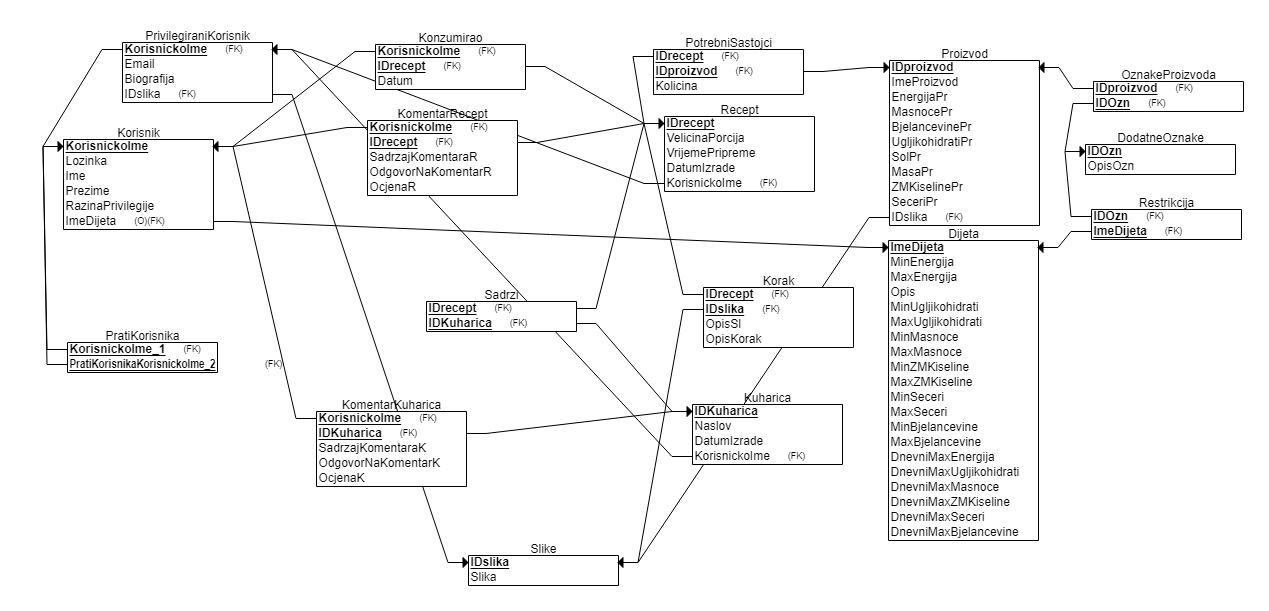
\includegraphics[scale=0.4]{slike/REL-model-baze.png}
					\caption{Relacijska shema baze podataka}
					\label{fig:REL-model-baze}
				\end{figure} 
			\eject
			
			
		\section{Dijagram razreda}
			\begin{figure}[H]
				\centering
				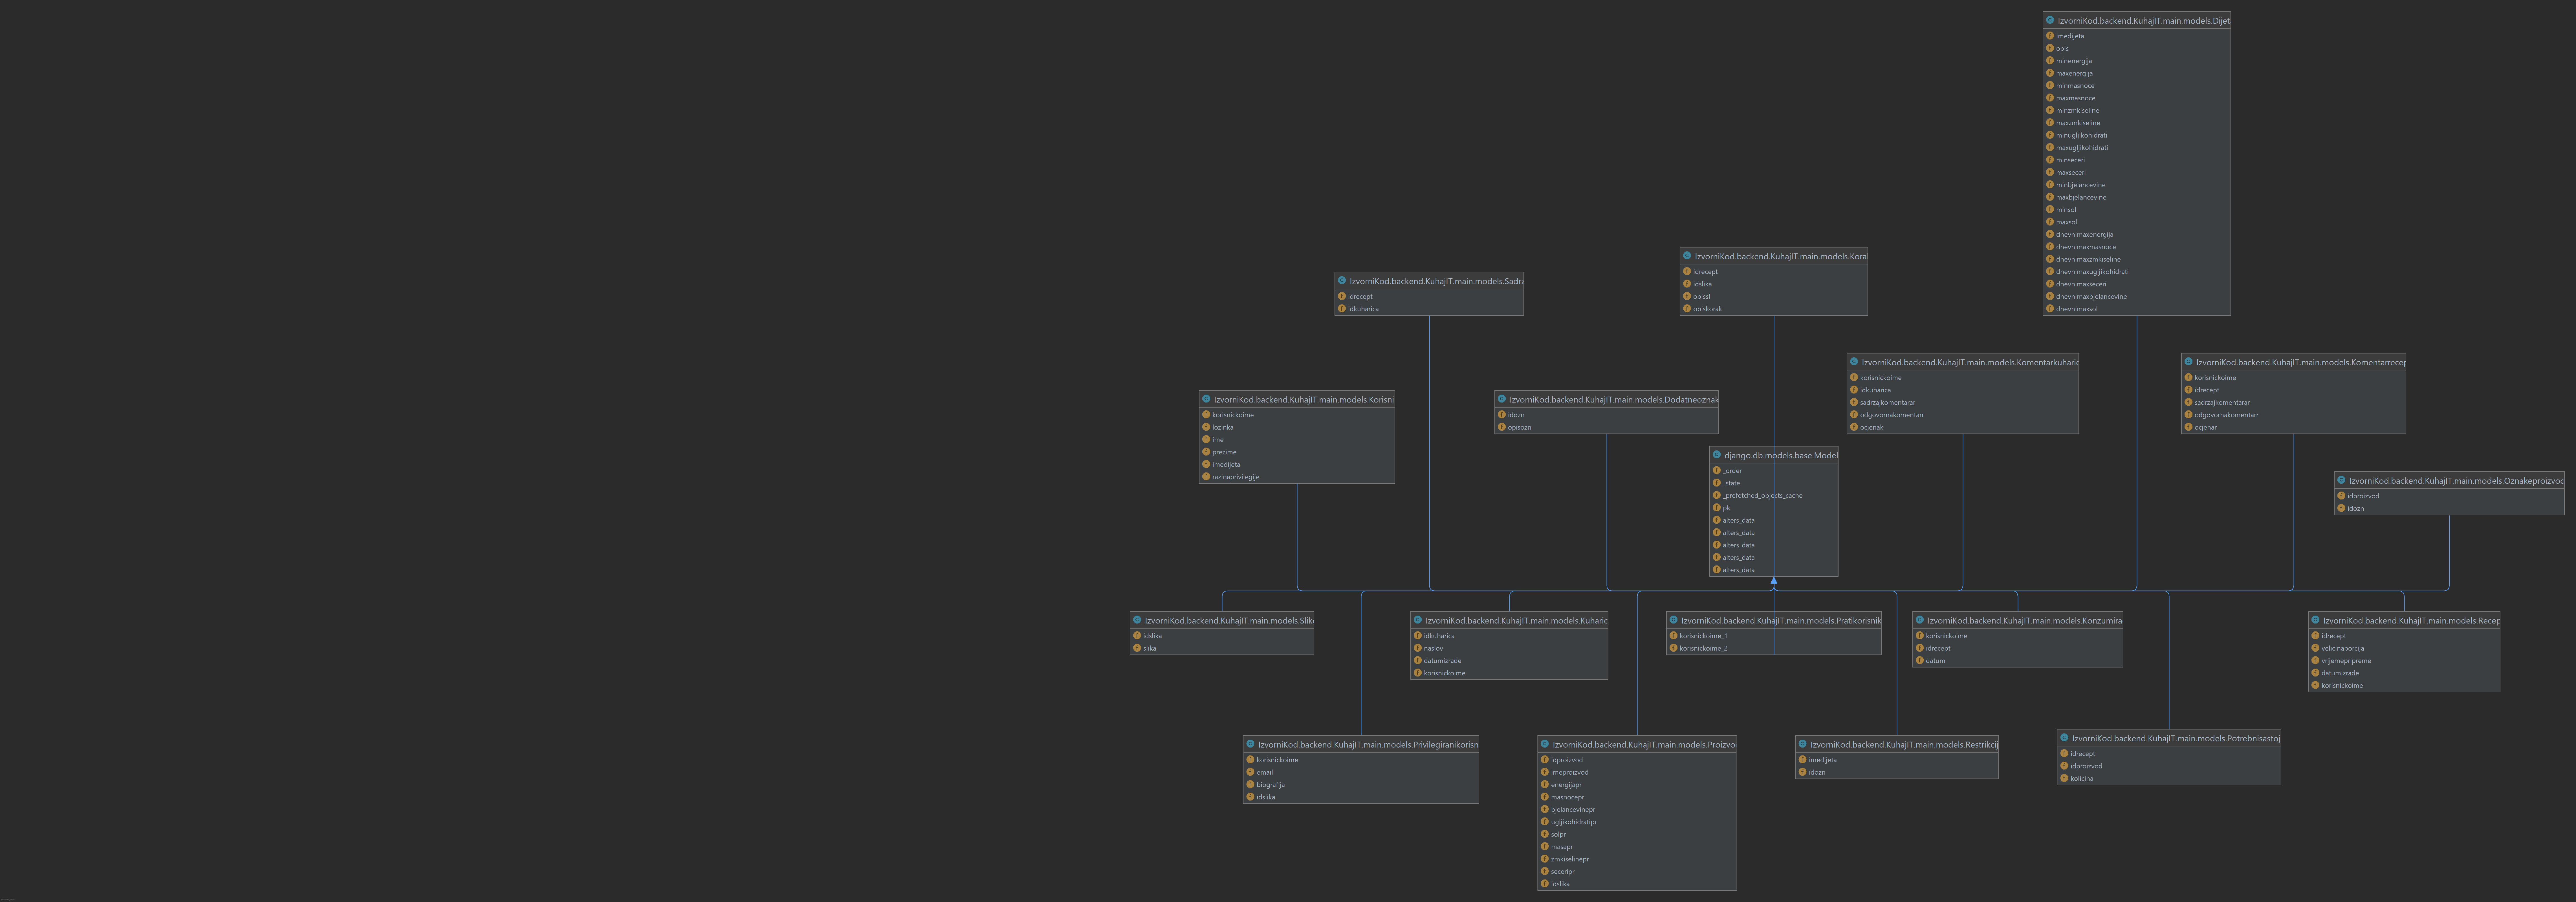
\includegraphics[scale=0.08]{dijagrami/dijagram-klasa.png}
				\caption{dijagram klasa}
				\label{fig:klase}
			\end{figure}
			%\textit{Potrebno je priložiti dijagram razreda s pripadajućim opisom. Zbog preglednosti je moguće dijagram razlomiti na više njih, ali moraju biti grupirani prema sličnim razinama apstrakcije i srodnim funkcionalnostima.}\\
			
			%\textbf{\textit{dio 1. revizije}}\\
			
			\textit{Prilikom prve predaje projekta, potrebno je priložiti potpuno razrađen dijagram razreda vezan uz \textbf{generičku funkcionalnost} sustava. Ostale funkcionalnosti trebaju biti idejno razrađene u dijagramu sa sljedećim komponentama: nazivi razreda, nazivi metoda i vrste pristupa metodama (npr. javni, zaštićeni), nazivi atributa razreda, veze i odnosi između razreda.}\\
			
			\textbf{\textit{dio 2. revizije}}\\			
			
			\textit{Prilikom druge predaje projekta dijagram razreda i opisi moraju odgovarati stvarnom stanju implementacije}
			
			
			
			\eject
		
		\section{Dijagram stanja}
			
			
			\textbf{\textit{dio 2. revizije}}\\
			
			\textit{Potrebno je priložiti dijagram stanja i opisati ga. Dovoljan je jedan dijagram stanja koji prikazuje \textbf{značajan dio funkcionalnosti} sustava. Na primjer, stanja korisničkog sučelja i tijek korištenja neke ključne funkcionalnosti jesu značajan dio sustava, a registracija i prijava nisu. }
			
			
			\eject 
		
		\section{Dijagram aktivnosti}
			
			\textbf{\textit{dio 2. revizije}}\\
			
			 \textit{Potrebno je priložiti dijagram aktivnosti s pripadajućim opisom. Dijagram aktivnosti treba prikazivati značajan dio sustava.}
			
			\eject
		\section{Dijagram komponenti}
		
			\textbf{\textit{dio 2. revizije}}\\
		
			 \textit{Potrebno je priložiti dijagram komponenti s pripadajućim opisom. Dijagram komponenti treba prikazivati strukturu cijele aplikacije.}